\capitulo{4}{Metodología}

\section{Descripción de los datos.}

En este trabajo, se emplean imágenes médicas de CXT frontal obtenidas a partir de un conjunto de datos público, algunas de ellas con neumonía y otras sin \footnote{\url{https://www.kaggle.com/datasets/paultimothymooney/chest-xray-pneumonia}}. Previamente a ser subidas a la plataforma correspondiente, todas las imágenes fueron examinadas minuciosamente de modo que, en primer lugar, todas aquellas imágenes que no tenían la calidad suficiente fueron descartadas. Después, dos médicos especializados evaluaron los diagnósticos de las imágenes asegurando que, estaban correctamente distribuidas en normal y neumonía y, por último, un tercer médico revisó la evaluación para evitar errores. Estas imágenes pertenecen a pacientes de entre 1 y 5 años. Se trata de imágenes con un formato .jpeg ~\cite{kaggle24}.

Para más información acerca de los datos consultar \textit{Anexo D}.
 
\section{Técnicas y herramientas.}

\subsection{Bibliotecas y herramientas empleadas}

\subsubsection{Anaconda}

Anaconda es una distribución de \textit{software} libre y comercial de lenguajes de programación Python y R, usada para la ciencia de datos y el aprendizaje automático ~\cite{wikianaconda24}. Permite la creación y gestión de entornos virtuales aislados, lo que ayuda a evitar conflictos entre diferentes versiones de paquetes. Se encuentra disponible para Windows, macOS y Linux, lo que la hace accesible a una amplia gama de usuarios ~\cite{anaconda24}.

\subsubsection{Python}

Python es un lenguaje de programación de alto nivel. Cuenta con un sistema de programación orientado a objetos ~\cite{Pyth24}. 

Entre sus beneficios, se puede destacar su eficiencia y su facilidad de uso gracias a una sintaxis clara y legible. Además, el \textit{software} es gratuito y se integra correctamente en todos los tipos de sistemas ~\cite{aws24}.

Para la realización de tareas, cuenta con una gran cantidad de bibliotecas, las cuales son de gran ayuda. Entre ellas se encuentra la biblioteca keras, la cual se emplea en este trabajo.

\subsubsection{Keras}

Keras es una biblioteca de redes neuronales profundas de código abierto escrita en Python ~\cite{wikikeras24}. Su objetivo es entrenar y compilar modelos de aprendizaje profundo.

Keras está integrada con TensorFlow, ya que es la API de alto nivel de esta plataforma por lo que, tiene acceso a todas las capacidades de esta multiplataforma ~\cite{TenFloKeras24}.

En este proyecto, se emplea esta herramienta para entrenar una arquitectura de aprendizaje automático basada en redes neuronales de forma rápida y eficiente. Estas redes determinarán la posible existencia de neumonía al realizar una radiografía.

\subsubsection{Tensorflow}

TensorFlow es una plataforma integral para el aprendizaje automático ~\cite{TenFlobasic24}.  Facilita la creación de modelos de aprendizaje automático de una forma sencilla ~\cite{TenFloint24}.

Esta biblioteca de código abierto permite el cálculo numérico basado en matrices multidimensionales. Además, es compatible con la diferenciación automática y la construcción, capacitación y exportación de modelos. Emplea la Unidad de Procesamiento Gráfico (GPU) para la realización del procesamiento distribuido, de forma que, múltiples computadoras o nodos trabajan simultáneamente para la realización de una tarea concreta o, de un conjunto de tareas ~\cite{TenFlobasic24}.

\subsubsection{LaTeX}

LaTeX es un editor de texto en línea, por lo que no requiere de ninguna instalación ni actualización de versiones. Cuenta con cientos de plantillas para comenzar a trabajar ~\cite{Over24}. Está orientado a la creación de documentos con una alta calidad topográfica ~\cite{CompHo24}.

Emplea un programa llamado motor TeX para el proceso de maquetación que se encarga de realizar de forma automática todo el aspecto visual del documento ~\cite{CompHo24}.

En este proyecto se ha empleado esta herramienta para la redacción de la memoria y los anexos.

\subsubsection{Kaggle}

Kaggle es una comunidad en línea de profesionales del aprendizaje automático y científicos de datos ~\cite{wikikaggle24}.

Es una plataforma que se emplea para buscar o publicar conjuntos de datos, resolver desafíos de ciencias de datos o emplear \textit{notebooks} con GPU integrado para no tener que emplear el ordenador local ~\cite{MaselData24}.

En este trabajo, se ha empleado esta plataforma para la obtención de las imágenes de CXT con y sin neumonía.

\subsubsection{GitHub y GitHub Desktop}

GitHub es una plataforma basada en la nube que cuenta con un sistema de control de versiones (VCS) llamado Git. Permite a los desarrolladores gestionar sus proyectos, realizar un seguimiento de los cambios en el código, colaborar con otros programadores y depositar sus repositorios de código ~\cite{HosTu24}. 

En este proyecto se ha empleado esta herramienta para la planificación de las distintas tareas realizadas, agrupando estas tareas en hitos (\textit{milestones}) y añadiéndoles etiquetas (\textit{labels}) para describirlas. Además, mediante ``GitHub Desktop'', una aplicación de escritorio gratuita, se ha clonado el repositorio del Trabajo de Fin de de Grado (TFG) de GitHub para sincronizar el código realizado en Python con las tareas estipuladas en ese repositorio.

\subsubsection{Scikit-learn}

Scikit-learn es una biblioteca de aprendizaje automático de código abierto para el lenguaje de programación Python ~\cite{wikisclearn24}.

Se trata de una herramienta simple y eficiente para el análisis predictivo de datos. Además, proporciona herramientas para la realización de diversas tareas como clasificación, regresión, agrupación, preprocesamiento, selección del modelo y reducción de dimensionalidad ~\cite{sclearn24}.

En este proyecto se ha empleado Scikit-learn para calcular alguna métrica más complicada como AUC y para la obtención de la matriz de confusión.

\subsubsection{Pandas}

Pandas es una biblioteca de Python empleada para la manipulación y análisis de datos de código abierto. Es una herramienta rápida, fácil de usar, potente y flexible ~\cite{pandas24}. 

Las dos estructuras principales de datos en pandas son DataFrame y Series. Un DataFrame es una tabla bidimensional de datos con filas y columnas etiquetadas. Y Series, es una estructura unidimensional de datos etiquetados. Permite realizar operaciones de indexación, selección, filtrado, agregación, y creación de gráficos de forma intuitiva y eficiente ~\cite{gamco24}.

En este caso, se ha empleado pandas para la obtención de DataFrames a la hora realizar diversas comparaciones.

\subsection{Alternativas de metodologías}
El objetivo de este trabajo es encontrar el mejor modelo de red neuronal para entrenar una serie de imágenes médicas y determinar si existe o no neumonía.

Se van a realizar diversas tablas comparativas entre distintos modelos, parámetros, etc. y, en cada una de ellas se escoge aquella opción que realiza el mejor entrenamiento y con la que se va a trabajar a partir de las siguientes comparaciones y así, sucesivamente.

\subsubsection{CNN propia}

En primer lugar, se realizó una CNN propia, basada en un ejemplo práctico disponible en Kaggle \footnote{\url{https://www.kaggle.com/code/paola311/clasificaci-n-de-im-genes-cnn}}. Esta CNN es bastante simple ya que, inicialmente no incluye capas ocultas, aunque, esto se modifica posteriormente creando nuevas arquitecturas con esta misma CNN pero incluyendo capas ocultas. 

La CNN inicial está compuesta por varias capas convolucionales (con las que se obtienen características importantes de las imágenes) seguidas de capas de MaxPooling2D para reducir la dimensionalidad. Después, se encuentra la capa Flatten, con la que se convierten las matrices de características en vectores y, por último, una capa densa para la clasificación binaria.

El objetivo de esta CNN es tener una primera evaluación del rendimiento del modelo que itere rápidamente y sirva de modelo base para, posteriormente, mejorar y ajustar los parámetros necesarios. Figura \ref{fig:cnn_propia}.

\begin{figure}[h]
    \centering
    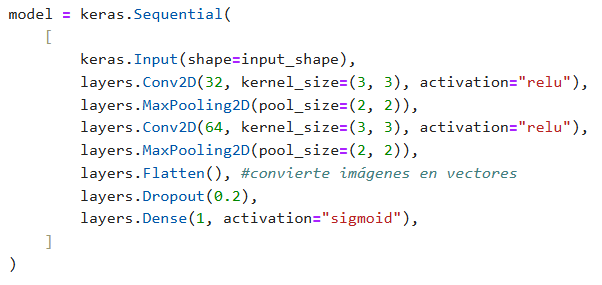
\includegraphics[width=0.99\textwidth]{img/cnn_propia.PNG}
    \caption{CNN propia. Fuente propia}
    \label{fig:cnn_propia}
\end{figure}


\subsubsection{CNN AlexNet}

La segunda CNN realizada está basada en la CNN AlexNet. AlexNet fue creada en 2012 por Alex Krizhevsky. Se trata de una red pre entrenada diseñada para reducir el error en la clasificación de imágenes para el proyecto ImageNet \cite{codificandobits24} (base de datos que proporciona una gran cantidad de imágenes etiquetadas para la IA \cite{datasmarts24}). Obtuvo muy buenos resultados de entrenamiento y supuso un gran avance en las arquitecturas de aprendizaje profundo \cite{diego23} aunque, al tratarse de una CNN muy profunda, requiere de un GPU (debido a su elevado coste computacional) y de una gran cantidad de datos para su correcto funcionamiento. 

Esta CNN está compuesta por cinco capas convolucionales. La primera, segunda y quinta capa convolucional están seguidas por una capa con la que se selecciona el máximo valor de un área (max-pooling) de 3×3 \cite{LMO24}. La primera capa convolucional incluye un filtro (\textit{kernal\_size})  de 11x11 y una reducción de dimensiones significativa (\textit{padding} = 4). En las siguientes capas convolucionales, el tamaño de filtro es menor (5×5 y 3×3) \cite{diego23}. Seguidamente, la CNN original de AlexNet contiene dos capas ocultas encargadas de la clasificación de las imágenes, de 4.096 neuronas cada una, y de una última capa densa de salida de 1.000 neuronas \cite{LMO24}. Figura \ref{fig:resumen_alexNet}. Pero, tanto las capas ocultas como la última capa densa han sido modificadas en este trabajo por tres modelos distintos con diferente número de capas ocultas.

\begin{figure}[h]
    \centering
    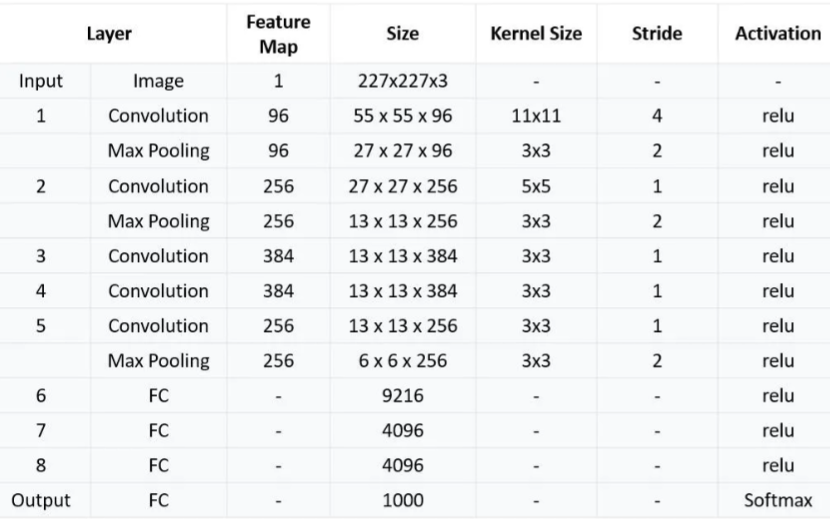
\includegraphics[width=0.99\textwidth]{img/resumen_alexNet.PNG}
    \caption{Resumen AlexNet. \cite{Medium24}}
    \label{fig:resumen_alexNet}
\end{figure}

\subsubsection{\textit{Batch size} y arquitectura}
En primer lugar, se han realizado dos tablas comparativas entre 3 arquitecturas de modelos diferentes y 4 valores de \textit{batch size} para la CNN propia y la CNN AlexNet.

La primera arquitectura se corresponde con un modelo que posee varias capas convolucionales (con las que se obtienen características importantes de las imágenes) seguidas de capas de MaxPooling2D para reducir la dimensionalidad. No posee capas ocultas. Finalmente se encuentra una capa densa de salida. 

De antemano ya se puede deducir que, este modelo es muy simple y, los resultados no van a ser buenos por lo que de descartará. Pero, así también se puede comprobar la mejora del modelo ajustándolo correctamente.

La segunda arquitectura se corresponde con un modelo que posee varias capas convolucionales (con las que se obtienen características importantes de las imágenes) seguidas de capas de MaxPooling2D para reducir la dimensionalidad. También hay una capa oculta de 100 neuronas y una capa densa de salida. 

La presencia de capas ocultas provoca una mejor capacidad para aprender de los datos del modelo ya que, al interconectarse la capa oculta con los datos de entrada, aprende características significativas de las características de entrada.

Por último, la tercera arquitectura, se corresponde con un modelo que posee varias capas convolucionales (con las que se obtienen características importantes de las imágenes) seguidas de capas de MaxPooling2D para reducir la dimensionalidad. En este caso, existen dos capas ocultas con 100 neuronas en la primera capa, y 16 neuronas en la segunda capa y, una capa densa de salida.

A su vez, se han probado 4 valores distintos (todos ellos potencias de 2) de \textit{batch size} para identificar el mejor modelo y el valor de \textit{batch size} con el que funciona mejor este modelo tanto con la CNN propia como con la CNN AlexNet.

Tal y como ya se ha comentado en los conceptos teóricos, el \textit{batch size} tiene un impacto importante en la precisión, velocidad y estabilidad del modelo y, dependiendo del objetivo puede funcionar mejor un \textit{batch size} u otro. Por eso, se busca determinar cuál es el ideal en este caso.

\subsubsection{Número de neuronas}
Una vez elegida la mejor CNN, el mejor modelo acorde a la arquitectura y el \textit{batch size}, se compara este modelo para distintos valores de neuronas en la capa oculta (todos estos valores son potencia de 2).

A mayor número de neuronas en la capa oculta, mejor se va a comportar la red con los datos de entrenamiento dado que, la capacidad de memorización de la red es mayor. Pero, peor se va a comportar con los datos de validación o prueba ya que no los ha visto ~\cite{diego23}. Por ello, es importante probar distintos valores y determinar cuál es el mejor para este caso.





